\section{Methodology}

\begin{figure*}[t]
    \centering
    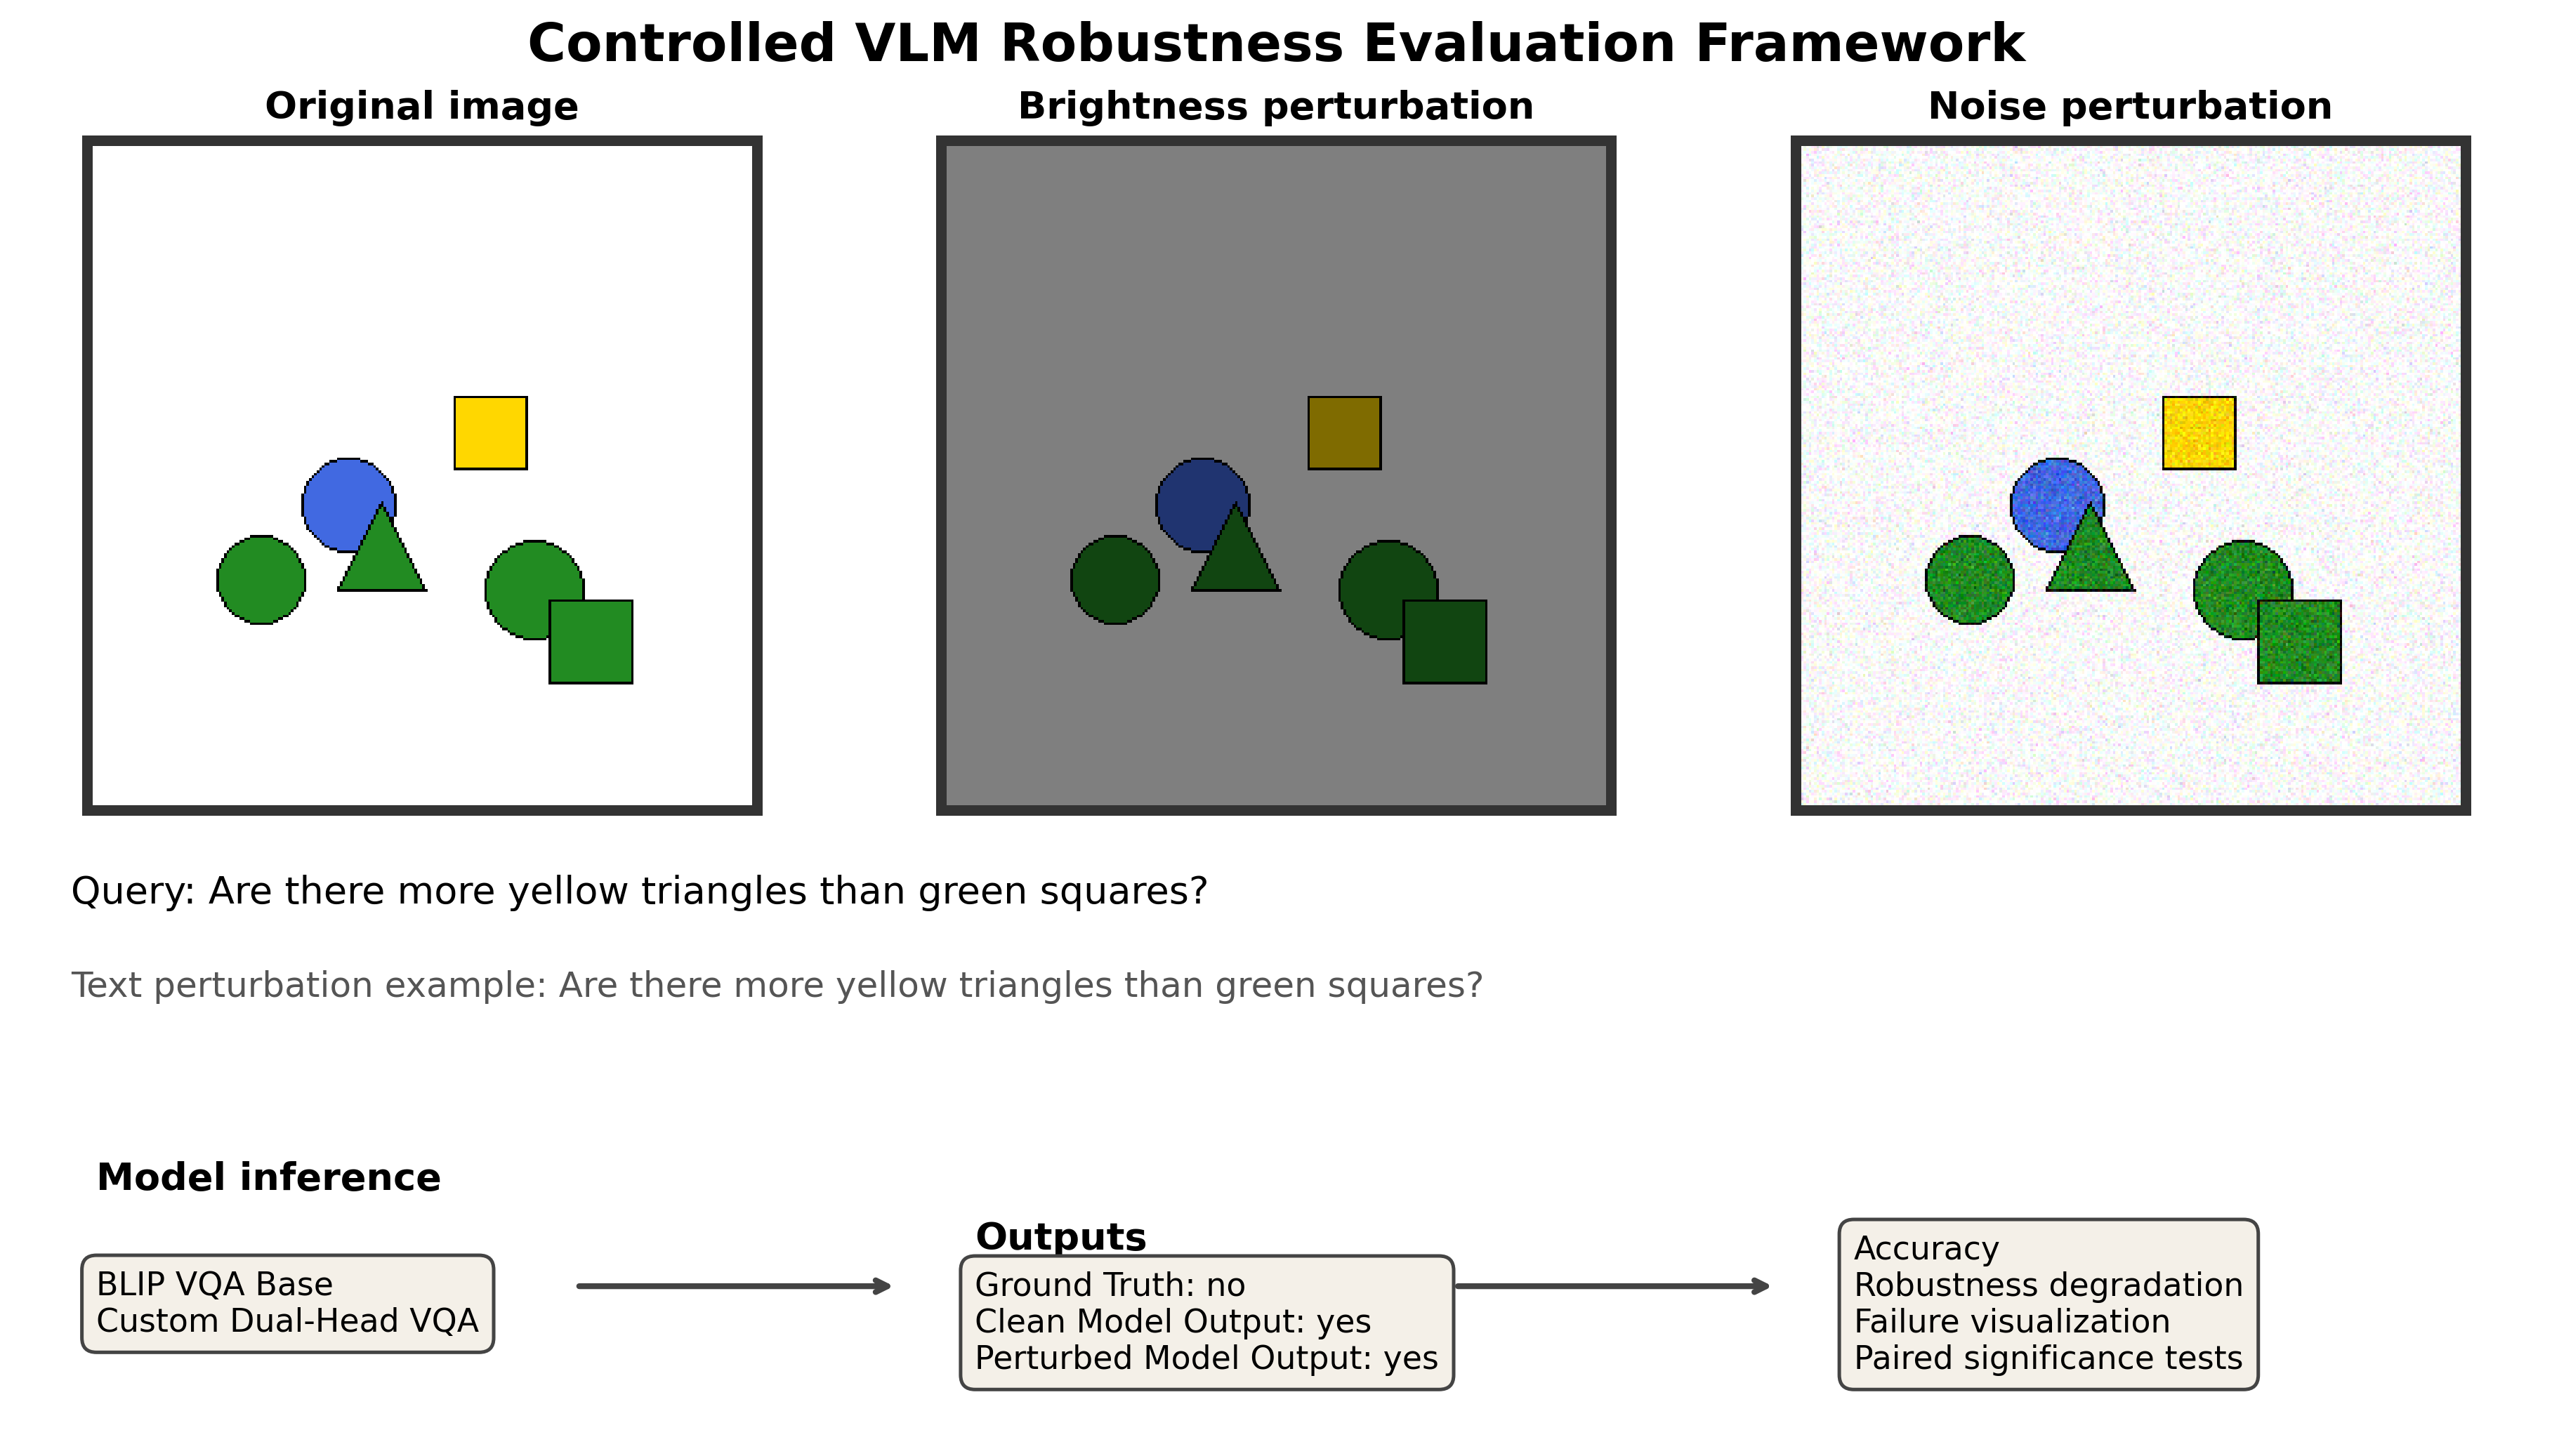
\includegraphics[width=0.95\textwidth]{figs/fig0_framework_overview.png}
    \caption{Overview of the controlled VLM robustness evaluation framework. The framework generates synthetic image-query pairs, applies semantic-preserving visual and textual perturbations, evaluates model outputs before and after perturbation, and records accuracy, robustness failures, and qualitative examples.}
    \label{fig:framework}
\end{figure*}

Our framework evaluates vision-language model robustness using controlled synthetic data. The goal is not to introduce a new state-of-the-art VLM, but to create a diagnostic setting where visual attributes, query semantics, perturbations, and ground-truth answers are precisely controlled. Figure~\ref{fig:framework} summarizes the full pipeline and shows the type of original and perturbed inputs used in the evaluation.

\paragraph{Synthetic data generation.}
Each image is a synthetic geometric scene rendered on a white background. Objects are sampled from a fixed set of colors and shapes: red, blue, green, and yellow; and circle, square, and triangle. Each scene contains a small number of randomly sampled objects, with object size and spatial position also randomized within the image canvas. The dataset stores both the rendered image and structured metadata for each object, including color, shape, position, and size. This metadata is used to automatically generate natural-language questions and exact ground-truth answers.

We evaluate four query types: \textit{existence}, \textit{counting}, \textit{spatial relationship}, and \textit{comparison}. Existence queries ask whether a target color-shape pair appears in the scene. Counting queries ask for the number of objects matching a target color and shape. Spatial queries ask whether one object is left of or above another object. Comparison queries ask whether one object category appears more frequently than another. These query types probe attribute binding, counting, and relational reasoning.

\paragraph{Perturbations.}
We apply three controlled perturbations while preserving the semantic answer. For brightness perturbation, image brightness is multiplied by a factor of 0.5. For noise perturbation, zero-mean Gaussian noise with standard deviation 20 is added independently to RGB pixel channels, and the resulting values are clipped to the valid image range. For text perturbation, the query is deterministically rephrased using hand-coded substitutions, such as replacing ``How many'' with ``What number of.'' These perturbations are designed to introduce controlled input variation without changing the correct answer.

\paragraph{BLIP baseline.}
The pretrained baseline is BLIP VQA Base, using the Hugging Face checkpoint \texttt{Salesforce/blip-vqa-base}. BLIP is an earlier vision-language model that combines a vision-transformer-based image encoder with transformer language components for visual question answering. Given an image and a question, the model conditions on both modalities and generates a short text answer. We use the checkpoint without fine-tuning, so BLIP serves as an inference-only pretrained baseline rather than a task-adapted model.

We use BLIP because it is lightweight enough to run reproducibly in a Colab T4 environment and provides a standard pretrained VQA comparison point. However, we do not claim that it represents the strongest current VLMs. Newer models such as Qwen2.5-VL or LLaVA-style systems would likely provide stronger general-purpose baselines, but evaluating them is left for future work.

\paragraph{Custom dual-head model.}
The custom model is a task-specific VQA classifier designed for the synthetic benchmark. It is not intended to be a general-purpose VLM. Instead, it provides a lightweight diagnostic baseline for testing whether simple task-specific structure helps under controlled reasoning tasks.

The model uses a ResNet-18 image encoder pretrained on ImageNet, with the final classification layer removed to produce a 512-dimensional image feature. The text query is tokenized using a word-level vocabulary and encoded with learned word embeddings followed by a bidirectional GRU. The final forward and backward GRU hidden states are concatenated to form the text feature.

The model also uses a learned query-type embedding for the four reasoning categories: existence, counting, spatial relationship, and comparison. The image feature, text feature, and query-type embedding are concatenated and passed through a shared multilayer perceptron to form a joint representation. This representation is then fed into two prediction heads. The yes/no head predicts a binary answer for existence, spatial, and comparison queries. The counting head treats counting as a multi-class classification problem over discrete count values observed in the dataset. Both heads are trained using cross-entropy loss.

This architecture is intentionally small. We use ResNet-18 and a GRU-based text encoder to isolate the effect of task-specific structure without relying on large-scale multimodal pretraining. The dual-head design reflects the different output spaces of yes/no reasoning and counting.

\paragraph{Evaluation metrics.}
Model outputs are normalized by lowercasing and stripping punctuation before exact string matching with the ground-truth answer. Accuracy is computed as the fraction of correctly answered examples. For each perturbation type, we define robustness degradation as
\[
\Delta = \mathrm{Acc}_{\mathrm{original}} - \mathrm{Acc}_{\mathrm{perturbed}}.
\]
Positive values indicate that performance decreases under perturbation, while negative values indicate that perturbed accuracy is slightly higher than original accuracy.

We also report per-query-type accuracy and automatically identify robustness failures. A robustness failure is defined as a case where the model answers correctly on the original input but incorrectly after a perturbation. Finally, we compare BLIP and the custom model using McNemar's exact test on paired predictions over the same test examples, together with bootstrap confidence intervals for paired accuracy differences.

\section{Experimental Settings}

The final dataset contains 3000 training-pool examples and 600 held-out test examples. For the custom model, 20\% of the training pool is used as a validation split for checkpoint selection. The held-out test set is used only for final evaluation. All reported BLIP and custom model results are computed on the same 600 test examples.

BLIP is evaluated in an inference-only setting using the checkpoint \texttt{Salesforce/blip-vqa-base}. No BLIP fine-tuning is performed. For each image-query pair, BLIP generates a short text answer, which is normalized and compared with the ground-truth answer.

The custom model is trained for 20 epochs using AdamW. The batch size is 64. We use a learning rate of $1 \times 10^{-5}$ for the pretrained ResNet-18 image encoder and $1 \times 10^{-3}$ for the task-specific layers, including the text encoder, query-type embedding, fusion MLP, and output heads. Weight decay is set to $1 \times 10^{-4}$. The model is trained using cross-entropy loss for both the yes/no head and the counting head.

During custom-model training, we apply data augmentation by randomly sampling from original inputs, brightness perturbations, noise perturbations, and text rephrasings. The best checkpoint is selected using validation accuracy. The best validation accuracy is 0.620, and the final clean test accuracy is 0.572.

All figures are generated programmatically from the saved prediction files. We report original accuracy, perturbed accuracy, robustness degradation, per-task accuracy, qualitative robustness failures, and paired statistical significance tests.

\section{Results}

\subsection{Overall Accuracy}

Table~\ref{tab:overall_accuracy} summarizes the overall accuracy of both models under original and perturbed inputs. BLIP achieves slightly higher accuracy on original inputs, while the custom model is competitive across all perturbation settings.

\begin{table}[t]
\centering
\caption{Overall accuracy under original and perturbed inputs.}
\label{tab:overall_accuracy}
\resizebox{\columnwidth}{!}{
\begin{tabular}{lcccc}
\toprule
Model & Original & Brightness & Noise & Text Rephrasing \\
\midrule
BLIP VQA Base & 0.593 & 0.590 & 0.570 & 0.570 \\
Custom Dual-Head VQA & 0.572 & 0.573 & 0.577 & 0.568 \\
\bottomrule
\end{tabular}
}
\end{table}

\begin{figure*}[t]
    \centering
    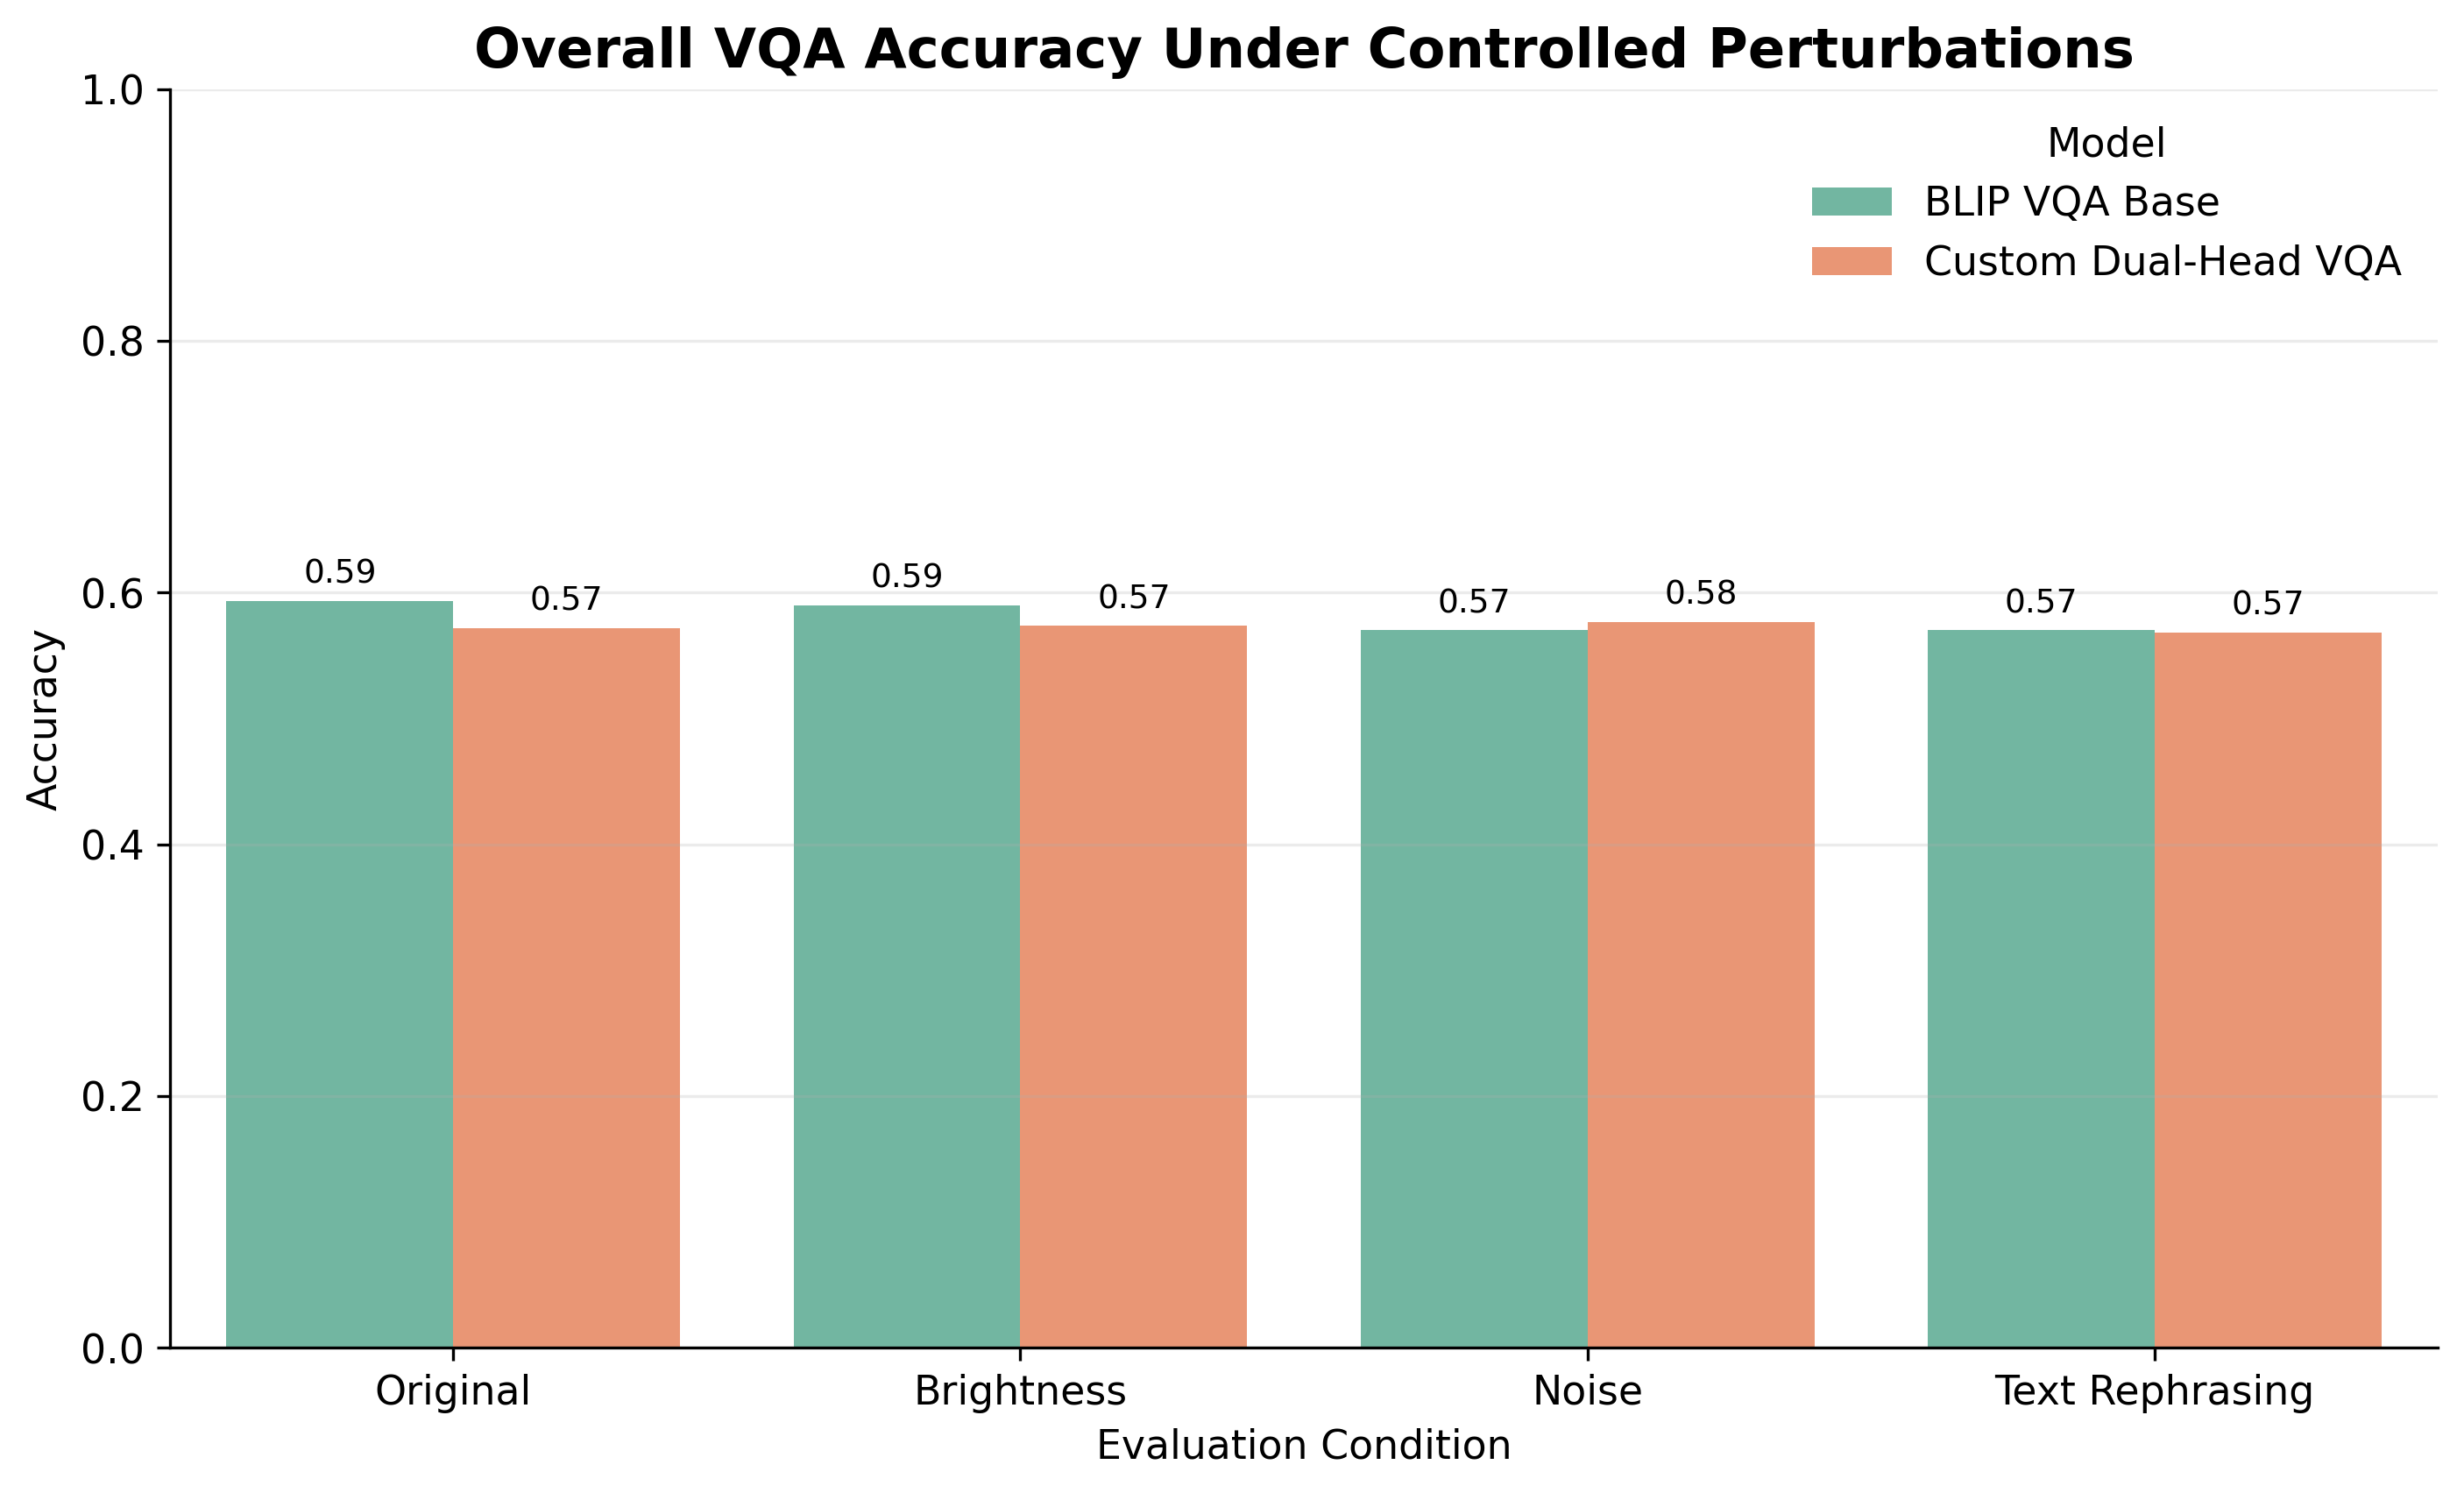
\includegraphics[width=0.72\textwidth]{figs/fig1_overall_accuracy_high_quality.png}
    \caption{Overall accuracy of BLIP and the custom dual-head model under original and perturbed inputs.}
    \label{fig:overall_accuracy}
\end{figure*}

Figure~\ref{fig:overall_accuracy} visualizes the same trend. BLIP performs best on original inputs, but the custom model remains close in overall accuracy. Under the noise perturbation, the custom model slightly exceeds BLIP. Since the custom model is trained with perturbation-based augmentation, this result is consistent with improved stability under controlled visual perturbations.

\subsection{Robustness Degradation}

\begin{figure*}[t]
    \centering
    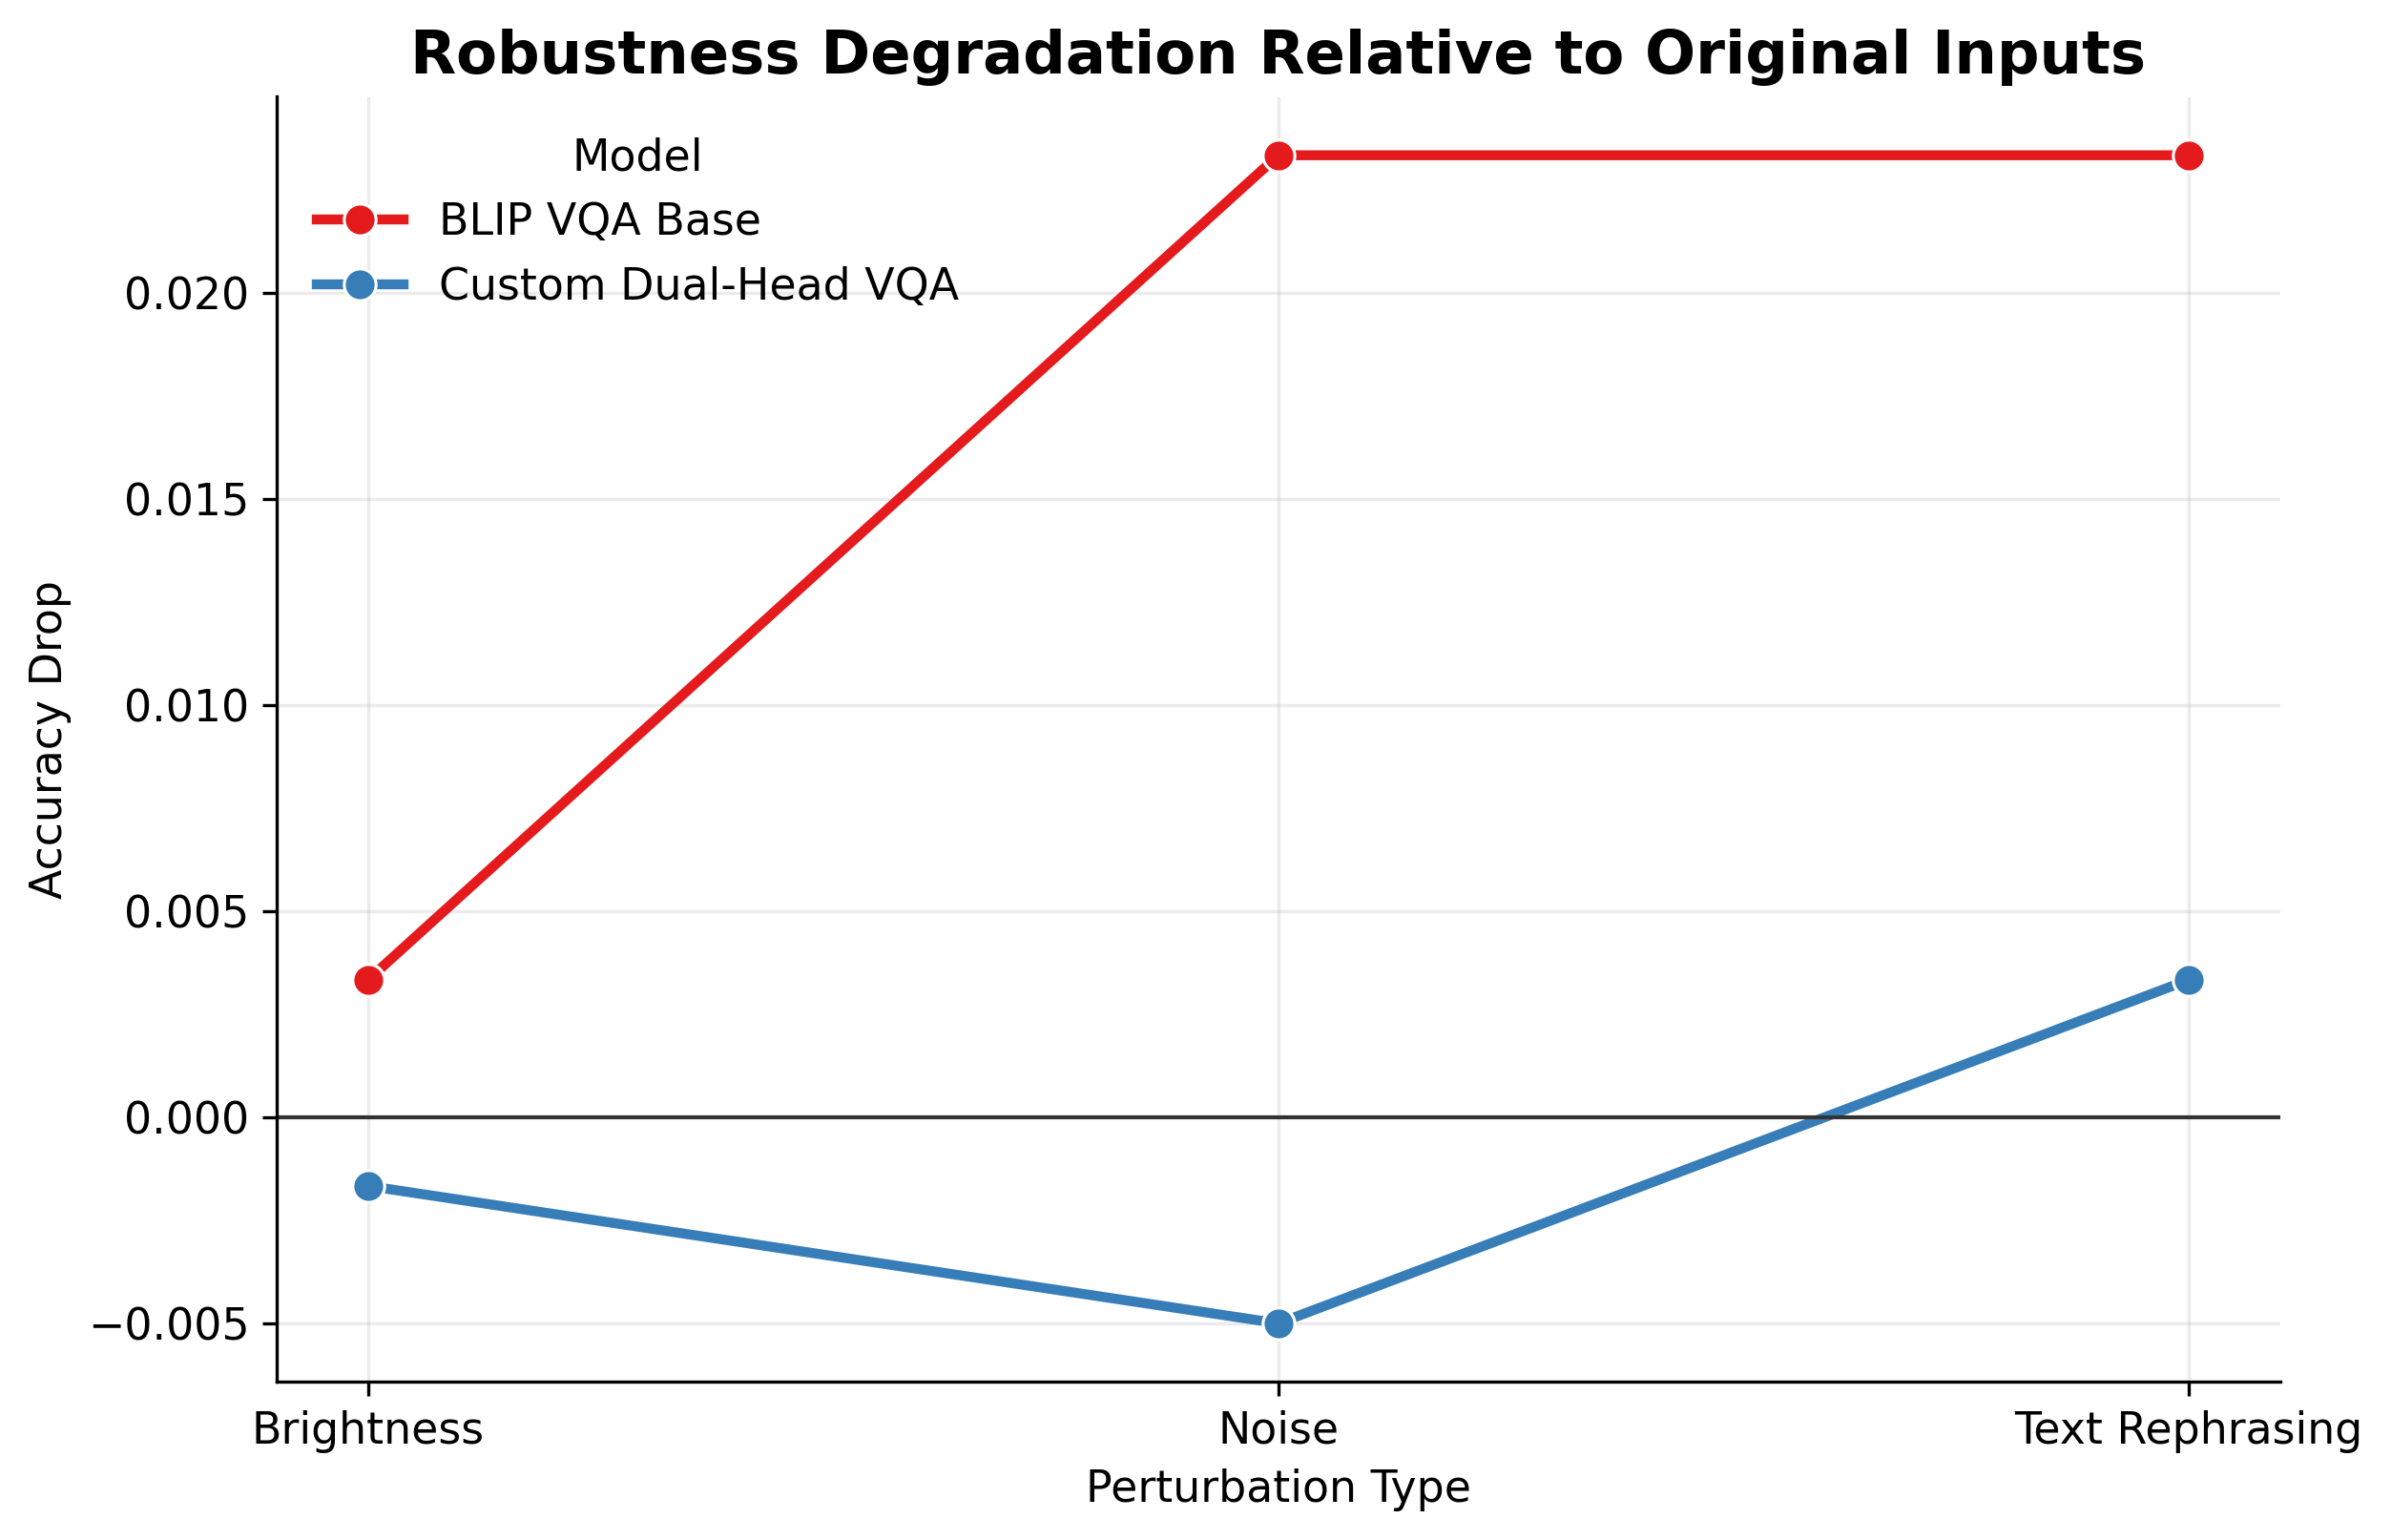
\includegraphics[width=0.72\textwidth]{figs/fig2_robustness_degradation.png}
    \caption{Robustness degradation relative to original inputs. Accuracy drop is computed as original accuracy minus perturbed accuracy. Values below zero indicate that perturbed accuracy is slightly higher than original accuracy.}
    \label{fig:robustness_degradation}
\end{figure*}

Figure~\ref{fig:robustness_degradation} shows robustness degradation for each perturbation. BLIP shows a small accuracy drop under all perturbations, especially noise and text rephrasing. The custom model shows very small changes across perturbations, with brightness and noise producing slightly higher accuracy than the original condition. These differences are small, so they should be interpreted as evidence of stability rather than large performance improvements.

\subsection{Per-Task Breakdown}

\begin{figure*}[t]
    \centering
    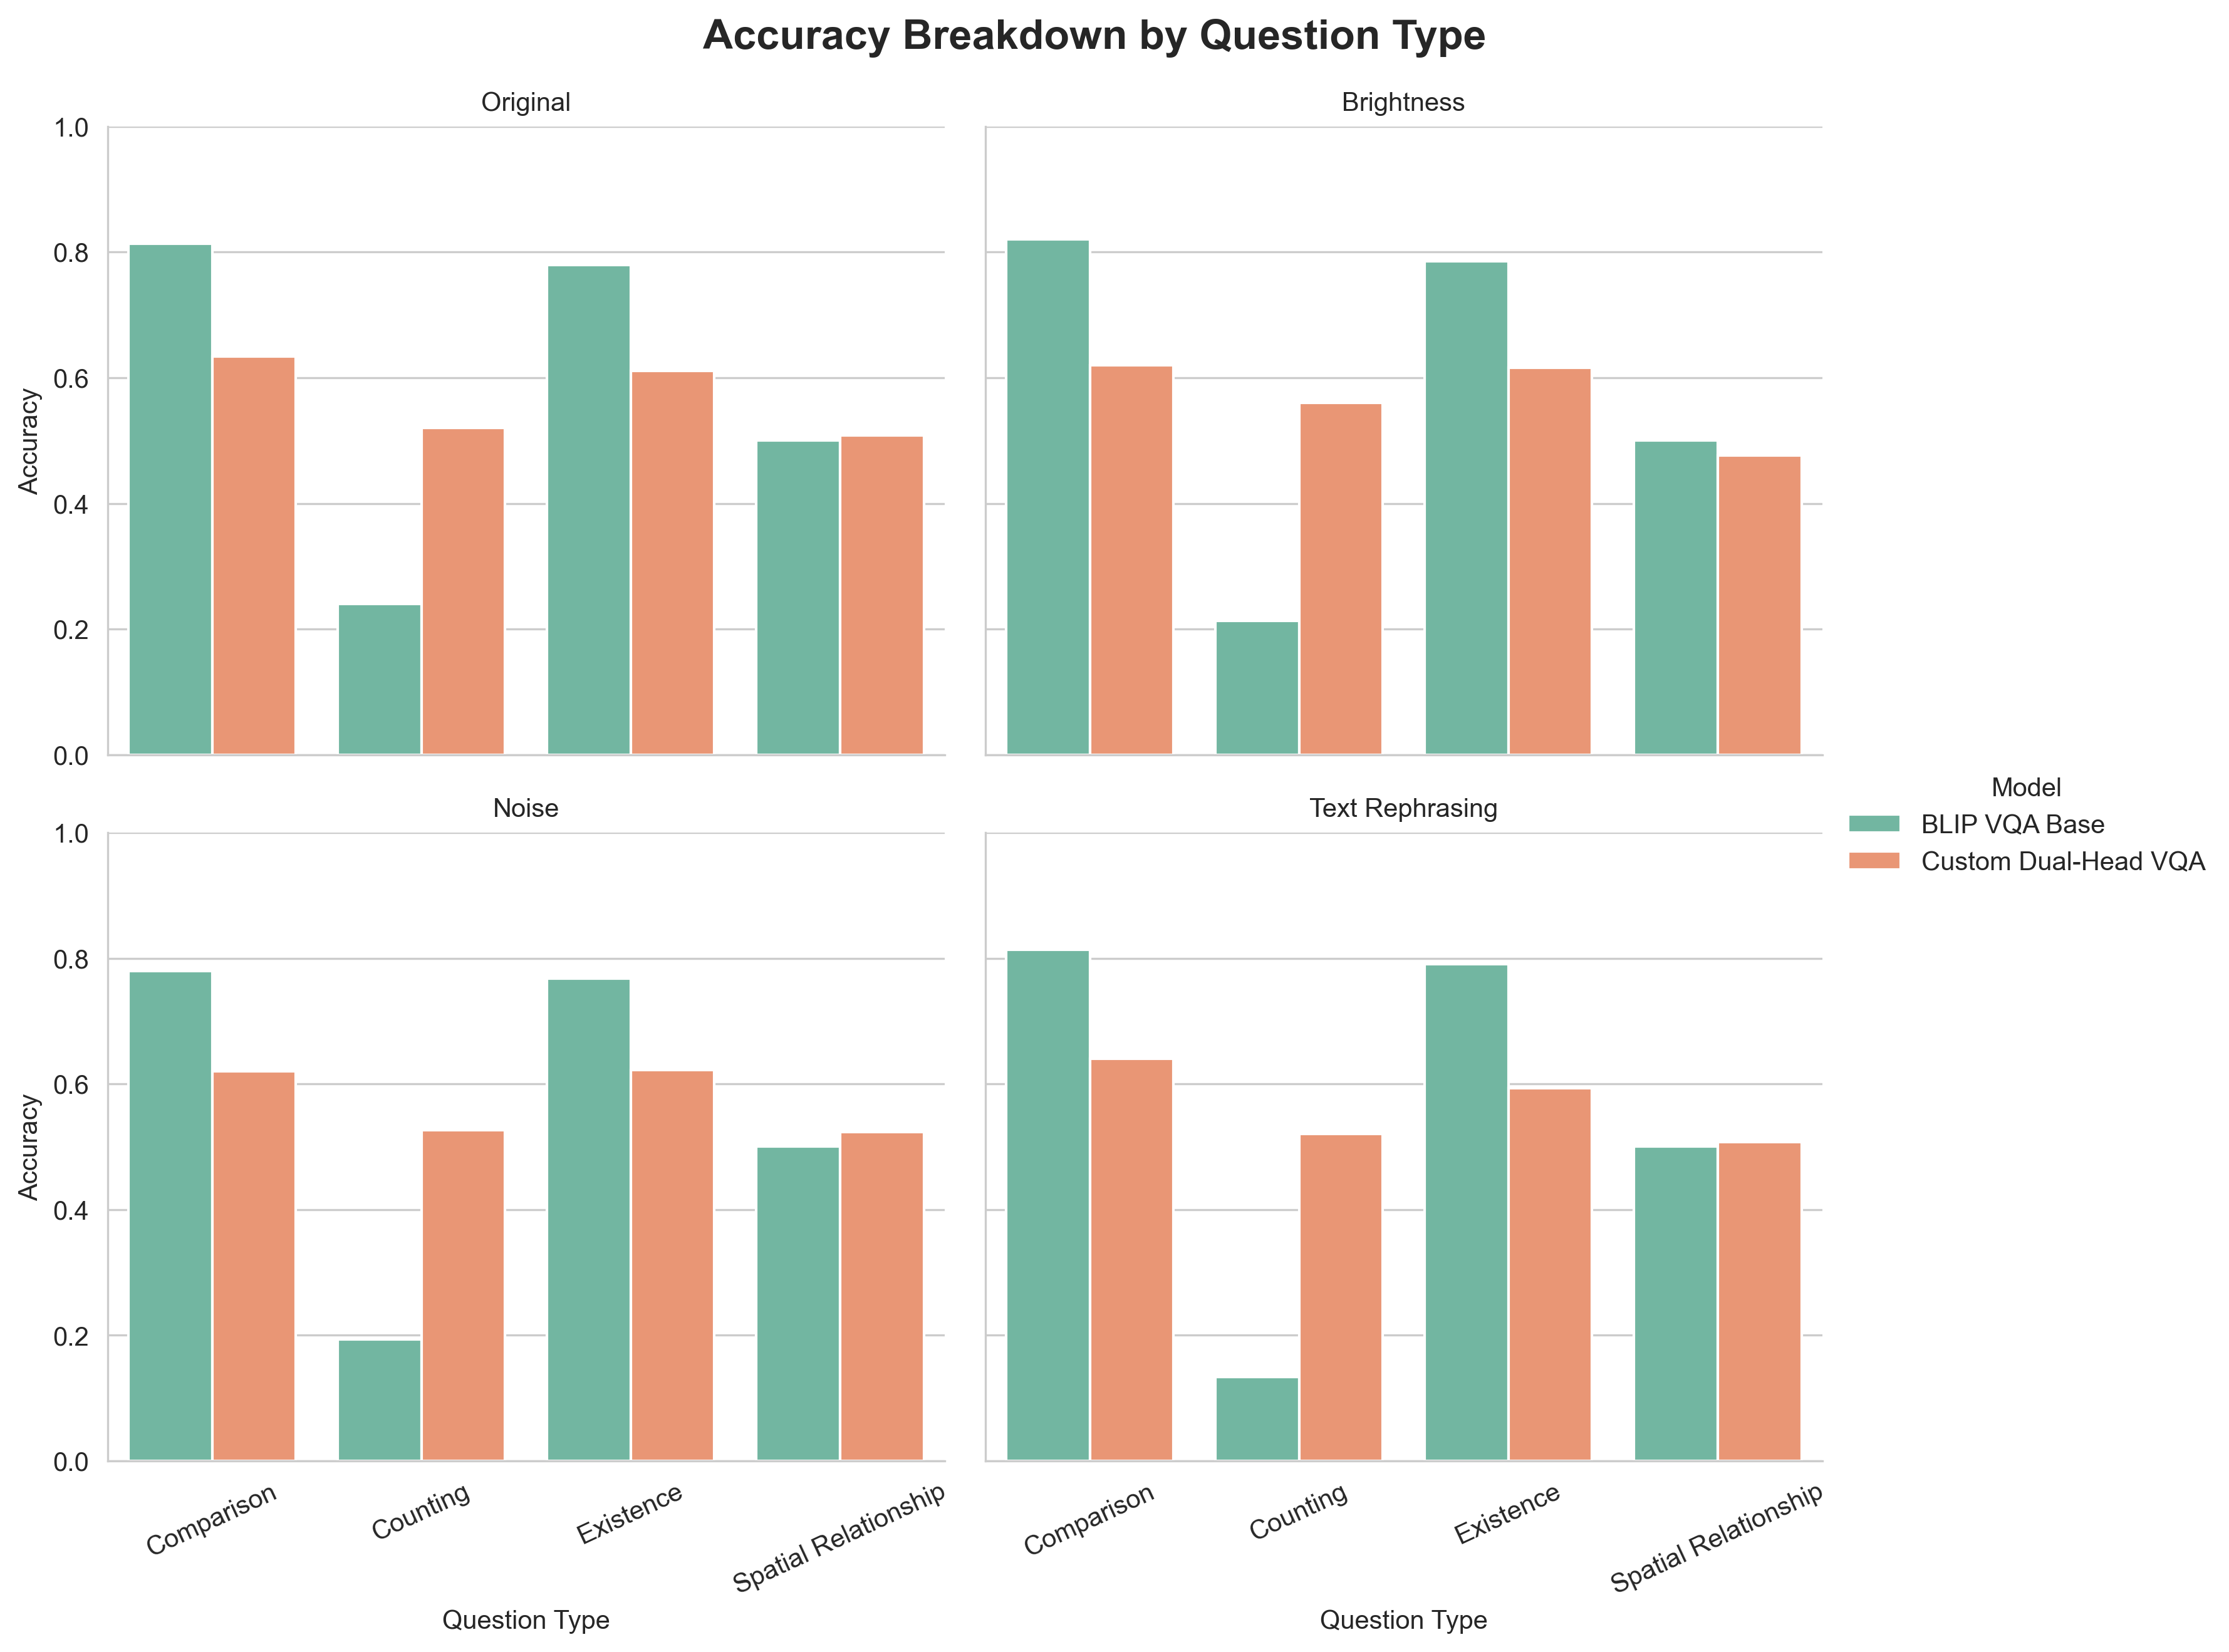
\includegraphics[width=0.72\textwidth]{figs/fig3_per_task_accuracy_breakdown.png}
    \caption{Accuracy breakdown by query type. BLIP performs strongly on existence and comparison queries but struggles with counting. The custom model improves counting performance but remains weaker on comparison and existence queries.}
    \label{fig:per_task}
\end{figure*}

Figure~\ref{fig:per_task} provides a finer-grained view across query types. BLIP performs well on existence and comparison queries, but counting remains difficult. In contrast, the custom model performs substantially better on counting than BLIP, reaching 0.520 original counting accuracy compared with BLIP's 0.240. This suggests that the task-specific count head helps on numerical questions. However, BLIP remains stronger on existence and comparison queries, likely due to its large-scale pretraining.

\subsection{Paired Statistical Comparison}

\begin{figure*}[t]
    \centering
    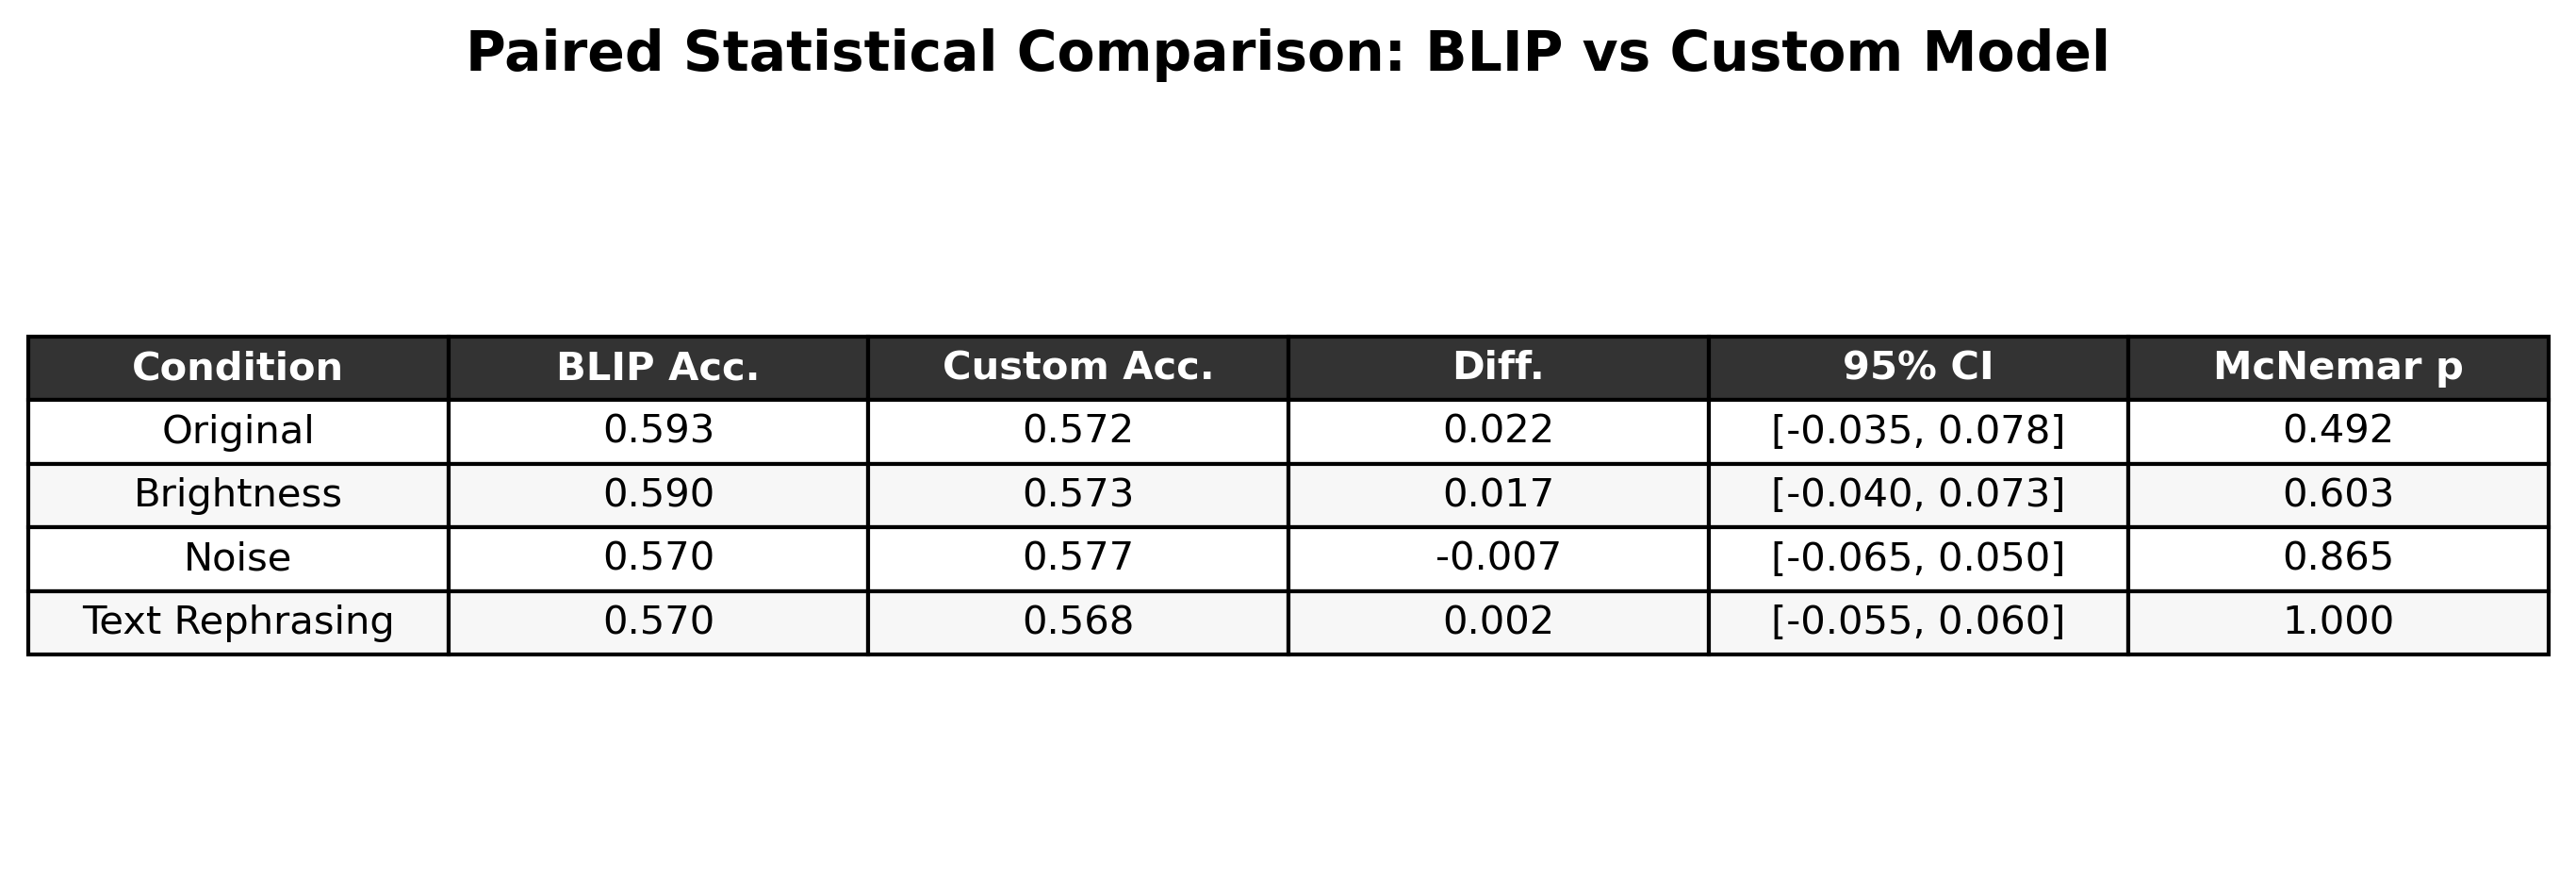
\includegraphics[width=0.72\textwidth]{figs/fig4_paired_significance_tests.png}
    \caption{Paired statistical comparison between BLIP and the custom model. McNemar's exact test is computed on paired predictions over the same 600 test examples. None of the differences are statistically significant at the 0.05 level.}
    \label{fig:significance}
\end{figure*}

Although BLIP has slightly higher original accuracy, paired statistical tests show that the differences between BLIP and the custom model are not statistically significant at the 0.05 level across all evaluation conditions. For original inputs, the BLIP-custom accuracy difference is 0.022 with a bootstrap 95\% confidence interval of $[-0.035, 0.078]$ and McNemar exact $p=0.492$. Under noise, the custom model is slightly higher, but the difference is also not significant ($p=0.865$). These results suggest that, under this controlled benchmark, the custom model is competitive with BLIP despite being much smaller and task-specific.

\section{Analysis and Discussion}

The results reveal several trends. First, aggregate accuracy alone hides important task-level differences. BLIP is stronger on existence and comparison questions, but it performs poorly on counting. The custom model, by contrast, benefits from its explicit count head and achieves better counting accuracy. This supports the idea that task-specific structure can improve performance on controlled reasoning tasks.

Second, perturbations affect the models differently. BLIP shows small but consistent degradation under brightness, noise, and text rephrasing. The custom model shows little overall degradation, and in some cases perturbed accuracy is slightly higher than original accuracy. Since the custom model is trained with random perturbation augmentation, this behavior is consistent with improved robustness to the perturbation types used during training.

Third, the paired significance analysis suggests that the overall difference between BLIP and the custom model is not statistically significant on this dataset. This does not mean the two models behave identically. Instead, the per-task results show complementary strengths: BLIP is better at some semantic recognition tasks, while the custom model is better at counting.

There are also important limitations. BLIP VQA Base is an older pretrained VQA model and should not be treated as representative of the strongest VLMs available in 2026. The custom model is trained from scratch for this benchmark and is best interpreted as a diagnostic baseline, not as a replacement for modern pretrained VLMs. The value of the experiment is therefore in the controlled evaluation framework, perturbation analysis, statistical comparison, and qualitative failure visualization rather than in claiming a new model architecture.

\subsection{Qualitative Failure Cases}

Quantitative plots are useful but do not fully explain how perturbations affect model behavior. To make the failures more interpretable, we visualize original and perturbed images side by side, along with the query, ground-truth answer, clean model output, and perturbed model output.

\begin{figure*}[t]
    \centering
    \includegraphics[width=0.48\textwidth]{figs/failure_cases/blip_vqa_base_text_failure_01_synthetic_vlm_test_00014.png}
    \hfill
    \includegraphics[width=0.48\textwidth]{figs/failure_cases/custom_dual-head_vqa_noise_failure_01_synthetic_vlm_test_00011.png}
    \caption{Representative robustness failures. Each example shows the original image, perturbed image, query, ground truth, clean model output, and perturbed model output. The left example shows a BLIP failure under text rephrasing, while the right example shows a custom model failure under noise.}
    \label{fig:failure_cases}
\end{figure*}

Figure~\ref{fig:failure_cases} shows representative robustness failures. These examples illustrate why visual inspection is important: a model may answer correctly on the original input but fail after a semantic-preserving perturbation. Such cases are not visible from bar charts alone. The failure visualizations also address the ambiguity of white-background synthetic images by adding explicit image borders.

Overall, the qualitative examples suggest that failures often arise from counting errors, attribute binding mistakes, or instability under input changes. Even when aggregate robustness degradation is small, individual examples show that predictions can change in ways that are inconsistent with the semantic content of the scene.

\section{Conclusion}

We presented a controlled evaluation framework for probing robustness in vision-language models using synthetic geometric scenes and semantic-preserving perturbations. The framework evaluates models under original, brightness, noise, and text-rephrased conditions, and reports aggregate accuracy, robustness degradation, per-task accuracy, paired statistical significance, and qualitative failure cases.

Our final experiments compare a pretrained BLIP VQA baseline with a lightweight custom dual-head VQA model. BLIP achieves slightly higher original accuracy, but the custom model becomes competitive after task-specific training and perturbation augmentation. The custom model performs especially well on counting compared with BLIP, while BLIP remains stronger on existence and comparison queries. Paired McNemar tests show that the overall accuracy differences are not statistically significant at the 0.05 level across evaluation conditions.

These results show that controlled synthetic evaluation can reveal behavior that is hidden by aggregate accuracy alone. In particular, per-task analysis and qualitative failure visualization are important for understanding when and why VLMs fail under perturbations. While the original project motivation included broader reliability measures such as calibration, the final system focuses on accuracy-based robustness, paired statistical testing, and interpretable failure analysis. Future work could extend this framework to newer pretrained VLMs, larger answer spaces, and calibration metrics based on comparable confidence estimates.
